\documentclass[12pt]{fphw}

\usepackage[utf8]{inputenc} % Required for inputting international characters
\usepackage[T1]{fontenc} % Output font encoding for international characters
\usepackage{mathpazo} % Use the Palatino font
\usepackage{graphicx} % Required for including images
\usepackage{booktabs} % Required for better horizontal rules in tables
\usepackage{amsmath}
\usepackage{hyperref}

\usepackage{xcolor}

\definecolor{codegreen}{rgb}{0,0.6,0}
\definecolor{codepurple}{rgb}{0.58,0,0.82}

\usepackage{listings} % for importing & highlighting code
\lstdefinestyle{mystyle}{
  commentstyle=\color{codegreen},
  keywordstyle=\color{blue},
  numberstyle=\tiny\color{codegray},
  stringstyle=\color{codepurple},  
  basicstyle=\ttfamily\footnotesize,
}
\lstset{style=mystyle}

\setlength{\parindent}{0in}

%----------------------------------------------------------------------
%	ASSIGNMENT INFORMATION
%----------------------------------------------------------------------

\title{Project}
\author{Aljaž Mur Eržen, Jakob Gaberc Artenjak}
\date{\today}
\institute{Faculty of computer and information science \\ Univerisity of Ljubljana}
\class{Big data}

%----------------------------------------------------------------------

\begin{document}

\maketitle

\section{Problem}

New York City Open Data is a website that contains many different datasets that are produced or in use by the city of New York, USA. One of the datasets, titled "Parking Violations Issued" \cite{violations-2021} contains information about 15M fines issued for parking violations for each of the years from 2014 onwards.

Our task was to handle the dataset, explore its contents and apply basics of machine learning, all while using big data approaches.

\section{Task 1: data formats}

To get started, we converted the dataset from its original CSV format to a few different formats and applied a few different compression algorithms to see, which format is the most suitable for use further on.

\begin{table}[h!]
\begin{center}
\begin{tabular}{l l r}
  Format & Compression & Size \\
  \hline
  parquet        & gzip                & 339 MB \\
  parquet        & brotli              & 398 MB \\
  avro           & snappy              & 662 MB \\
  parquet        &                     & 671 MB \\
  avro           &                     & 2.2 GB \\  
  HDF            & zlib, comp. level=9 & 2.2 GB \\
  CSV (original) &                     & 2.2 GB \\
  HDF            &                     & 2.6 GB \\
\end{tabular}
\caption{Comparison of sizes produced by different storage formats}
\label{table-formats}
\end{center}
\end{table}

One can see that HDF is not efficient at all. Without compression, the size of the dataset actaully grew when converted from plain-text CSV. 

Most efficient format was parquet with gzip compression, which produced not only the smallest output, but has also been comparable to other formats in terms of time required for the compression.

Parquet is a file format developed by Apache Fundation. It stores tabular data, organized in rows and columns, but contrary to CSV and most relational databases, it does not store data by rows, but by columns. This approach is called columnar storage and is beneficial because of the fact that usually, values in the same column are more similar than values in the same row, which may differ even in their data type. 

\section{Task 2: augemtation}

Our current data is unclean and insufficient for proper data extraction. In order to improve our data we decided to create a process which filters, phrases and corrects our data for further tasks.

There are a total of seven augmentations. We also filter the columns to save on space, however this is not explicitly part of any of the augmentations.

\subsection{Augmentation: address}

In this augmentation we attempt to find the locations of each ticket. Firstly we match each ticket each tickets street code and house number to those in the NYC property address directory\cite{bobaadr} and append data about the BIN (building identification number), the physical id of the building, and the zip code.

Secondly we match the BIN and the psychical id with the NYC address points\cite{address_point} data in order to obtain the street name, the longitudes and latitudes, and the borough.

\subsection{Augmentation: cafes}

We found data details the locations of cafes in NYC\cite{cafes}. Through the previously obtained zip codes we append information about the number of cafes near the incident of the ticket (specifically, number of cafes on registered on the zip code).

\subsection{Augmentation: violation}

Through the help of data which describes the price of each ticket (which can be found as an attachment at the NYC parking violations data\cite{violations-2021}) we augmented the data with the price of the ticket. This is done with the help of the violation code that is in the original data.

\subsection{Augmentation: car\_color}

Due to the car color data being dirty (different names for the same color or unreadable entries) we decided to clean it up. We made a list of what we assume each color in the data means and applied it on the data.

\subsection{Augmentation: ticket\_datetime}

The time of each ticket is given in two different columns. We used a function which combined those columns and gave us a new column with the datetime format for easier processing.

Some tickets have the year set to something outside of the year of the dataset. We corrected this so all tickets in a dataset have the year of the dataset.

\subsection{Augmentation: weather}

With the help of a weather API\cite{weatherr} we obtained some weather information to add to our data. This information includes average daily temperature, humidity, snow depth, wind speed and description.

We only have the daily averages since the amount of calls needed for the hourly measurements make it harder to obtain.



\subsection{Augmentation: school}

With the help of the list of schools in NYC\cite{school} and the previously obtained longitude and latitude of each ticket we added the closest school for each ticket. We added the school district, the location code and the name of the school to our data.

\subsection{Filtering columns}

Our final data has the columns: 
Vehicle body type, vehicle maker, vehicle year, zip code, borough code, street name, longitude, latitude, number of cafes on the same street, violation price, vehicle color, the time of the ticket, average daily temperature, humidity, snow depth and wind speed, weather description, and name of the closest school.


\section{Task 3: exploration}

We can see some of the ticket locations in the figure\ref{fig:map_1}.

\begin{figure}[h!]
  \label{fig:map_1}
  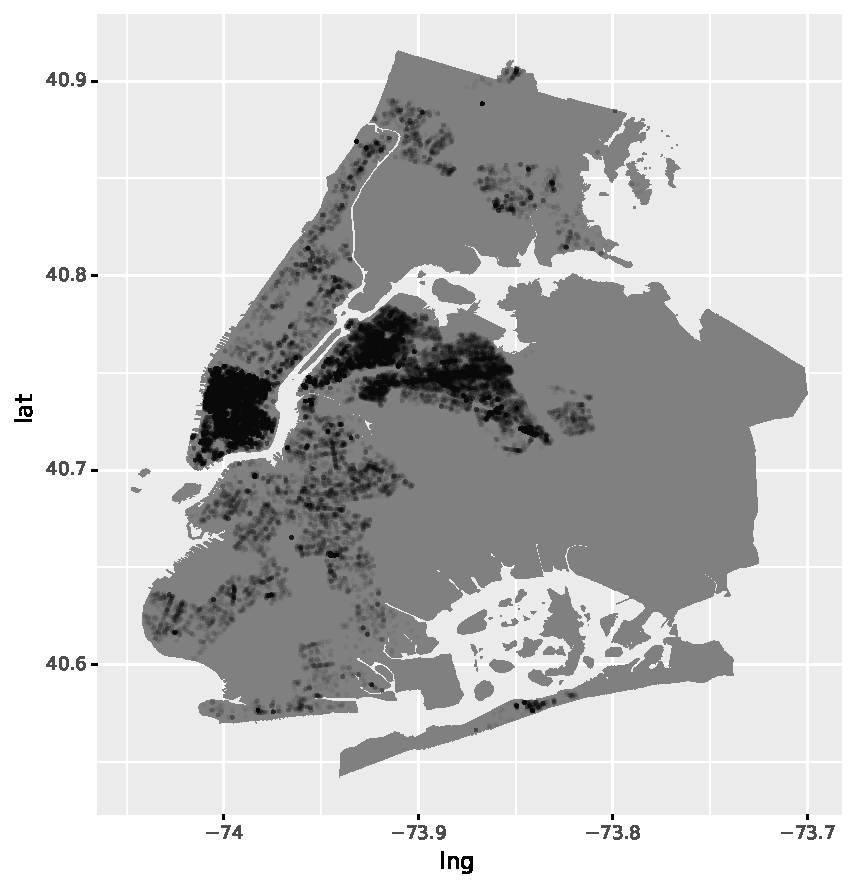
\includegraphics[width=1\textwidth]{figures/nyc.map.png}
  \caption{Locations of violations in the year 2022 in the months January to May}
\end{figure}

We wanted to know which color of cars gets the most amount of tickets. A graph of number of tickets per car color can be seen in figure\ref{fig:color_1}. This does not tell us much, as we do not know the total amount of cars of a given color. Following up on this we decided to calculate the mean and standard deviation of violation prices for cars of a given color. This graph can be seen in figure\ref{fig:color_2}.
There seem to be three major outliers wrt amount of tickets for a given color, those being black, white and gray. This is to be expected, as those car colors are quite common. It is interesting to see that gray and black have a low mean violation price, but white has a medium mean violation price. The highest violation price goes to brown.

\begin{figure}[h!]
  \label{fig:color_1}
  \includegraphics[width=1\textwidth]{figures2/VehicleColor_count.png}
  \caption{The number of tickets for cars of a particular color from year 2015 to 2022}
\end{figure}

\begin{figure}[h!]
  \label{fig:color_2}
  \includegraphics[width=1\textwidth]{figures2/VehicleColor_price.png}
  \caption{The mean and standard deviation of violation price for cars of a particular color from year 2015 to 2022}
\end{figure}

We made the same statistics for the vehicle body type. The graph for the number of tickets can be seen in figure\ref{fig:type_1} while the mean and standard deviation of ticket price can be seen in figure\ref{fig:type_2}.
While we don't know enough vehicle body types to make any solid conclusions based on this data it can be seen from the mean price that there are bigger differences between them. This is expected, as we would imagine that certain vehicles can be more problematic in traffic due to the differences in size.

\begin{figure}[h!]
  \label{fig:type_1}
  \includegraphics[width=1\textwidth]{figures2/VehicleBT_count.png}
  \caption{The number of tickets for cars of a particular type from year 2015 to 2022}
\end{figure}

\begin{figure}[h!]
  \label{fig:type_2}
  \includegraphics[width=1\textwidth]{figures2/VehicleBT_price.png}
  \caption{The mean and standard deviation of violation price for cars of a particular type from year 2015 to 2022}
\end{figure}

We've done the same for the vehicle maker. The count of tickets per vehicle maker can be seen in figure\ref{fig:maker_1} and the graph for the mean violation price can be seen in figure\ref{fig:maker_2}.
There are a few vehicle makers which stand out wrt number of tickets, though the same issue presists; how many vehicles of a certain maker does exist? We do not know. Though we can see there are five outliers in the mean violation price. Those being ISUZU, INTER, HIN, FRUCH, and NS/OT. Looking back at how many ticket each vehicle maker amasses it seems like all four of those are on the lower end except FRUCH, which is seems to have a bit more tickets.

\begin{figure}[h!]
  \label{fig:maker_1}
  \includegraphics[width=1\textwidth]{figures2/VehicleMaker_count.png}
  \caption{The number of tickets for cars of a particular maker from year 2015 to 2022}
\end{figure}

\begin{figure}[h!]
  \label{fig:maker_2}
  \includegraphics[width=1\textwidth]{figures2/VehicleMaker_price.png}
  \caption{The mean and standard deviation of violation price for cars of a particular maker from year 2015 to 2022}
\end{figure}


We've made the same two graphs for vehicle year. The count graph is in figure\ref{fig:year_1} while the mean violation price is in figure\ref{fig:year_2}. There is a gap in the year 2000. We are unsure why that is.
As expected more cars are from the recent years rather than being older. The mean violation price is similar for newer models but seems to spike around the year 1990.

\begin{figure}[h!]
  \label{fig:year_1}
  \includegraphics[width=1\textwidth]{figures2/VehicleYear_count.png}
  \caption{The number of tickets for cars of a particular year of registration from year 2015 to 2022}
\end{figure}

\begin{figure}[h!]
  \label{fig:year_2}
  \includegraphics[width=1\textwidth]{figures2/VehicleYear_price.png}
  \caption{The mean and standard deviation of violation price for cars of a particular year of registration from year 2015 to 2022}
\end{figure}

We also have the same two graphs for boroughs. The count graph is in figure\ref{fig:borough_1} while the mean violation price is in figure\ref{fig:borough_2}.
It seems as if there are more violations happening in Manhattan compared to other borough. This can partly be seen in our visualized data at the start of this chapter\ref{fig:map_1}. Even though the uneven violations across boroughs it seems that the mean prices are not too far apart.


\begin{figure}[h!]
  \label{fig:borough_1}
  \includegraphics[width=1\textwidth]{figures2/Borough_count.png}
  \caption{The number of tickets for each borough from year 2015 to 2022}
\end{figure}

\begin{figure}[h!]
  \label{fig:borough_2}
  \includegraphics[width=1\textwidth]{figures2/Borough_price.png}
  \caption{The mean and standard deviation of violation price for each borough from year 2015 to 2022}
\end{figure}


We also decided to make some analysis based on the impact of weather to the violations price.
Firstly we'd like to show the number of tickets for each month in figure\ref{fig:month_c} and the average violation price for each month in figure\ref{fig:month_p}.

\begin{figure}[h!]
  \label{fig:month_c}
  \includegraphics[width=1\textwidth]{figures2/Month_count.png}
  \caption{The number of tickets for each month from year 2015 to 2022}
\end{figure}

\begin{figure}[h!]
  \label{fig:month_p}
  \includegraphics[width=1\textwidth]{figures2/Month_price.png}
  \caption{The mean and standard deviation of violation price for each month from year 2015 to 2022}
\end{figure}



While the number of tickets fluctuates based on the month the violation price does not.
We want to see how the average daily temperature, humidity, and snow depth change for tickets of each specific months. This can be seen in figures\ref{fig:month_t}\ref{fig:month_h}\ref{fig:month_s} respectively.
The changes in temperature are as we'd expect, its hotter in the summer and cooler in the winter. The humidity seems to be the highest during fall and lowest during spring. The snow depth is generally zero outside of winter.
Since we didn't notice any changes in the count and price graph for each month it is hard to conclude any reasonable connection them between temperature, humidity and snow depth.


\begin{figure}[h!]
  \label{fig:month_t}
  \includegraphics[width=1\textwidth]{figures2/Month_temp.png}
  \caption{The average temperature for each month from year 2015 to 2022}
\end{figure}

\begin{figure}[h!]
  \label{fig:month_h}
  \includegraphics[width=1\textwidth]{figures2/Month_humidity.png}
  \caption{The average humidity for each month from year 2015 to 2022}
\end{figure}

\begin{figure}[h!]
  \label{fig:month_s}
  \includegraphics[width=1\textwidth]{figures2/Month_snowdepth.png}
  \caption{The average snow depth for each month from year 2015 to 2022}
\end{figure}


Never the less we decided to again figure out the impact of temperature, humidity and snow depth on the Violation price.
We made the count and price graphs for all three of them. The graphs for temperature can be found in figures\ref{fig:month_tc}\ref{fig:month_tp}, the graphs for humidity in figures\ref{fig:month_hc}\ref{fig:month_hp}, and the graphs for snow depth in figures\ref{fig:month_sc}\ref{fig:month_sp}.

\begin{figure}[h!]
  \label{fig:month_tc}
  \includegraphics[width=1\textwidth]{figures2/Temp_count.png}
  \caption{The number of tickets for each rounded temperature value from year 2015 to 2022}
\end{figure}

\begin{figure}[h!]
  \label{fig:month_tp}
  \includegraphics[width=1\textwidth]{figures2/Temp_price.png}
  \caption{The mean and standard deviation of violation price for each rounded temperature value from year 2015 to 2022}
\end{figure}

\begin{figure}[h!]
  \label{fig:month_hc}
  \includegraphics[width=1\textwidth]{figures2/Humidity_count.png}
  \caption{The number of tickets for each rounded humidity value from year 2015 to 2022}
\end{figure}

\begin{figure}[h!]
  \label{fig:month_hp}
  \includegraphics[width=1\textwidth]{figures2/Humidity_price.png}
  \caption{The mean and standard deviation of violation price for each rounded humidity value from year 2015 to 2022}
\end{figure}

\begin{figure}[h!]
  \label{fig:month_sc}
  \includegraphics[width=1\textwidth]{figures2/Snowdepth_count.png}
  \caption{The number of tickets for each rounded snow depth value from year 2015 to 2022}
\end{figure}

\begin{figure}[h!]
  \label{fig:month_sp}
  \includegraphics[width=1\textwidth]{figures2/Snowdepth_price.png}
  \caption{The mean and standard deviation of violation price for each rounded snow depth value from year 2015 to 2022}
\end{figure}

We can see that the number of tickets is somewhat evenly spread except of the outliers. And so is the price except for $-13$ which we assume is high due to small amount of tickets being done at that temperature. We can assume that temperature does not have much of an impact on the resulting violation price.

Humidity has more of a bell curve count wise, though the average price is also quite evenly spread. Humidity does not have much of an impact on the resulting violation price.

Snow depth have the most tickets close to 0, which is expected. What we can see is that the violation price does change when the snow depth increases. There seems to be an outlier somewhere around 170 snow depth, which we assume is an error in the weather API.


\section{Task 4: streaming}

Due to the nature of this task it is hard to show any results as a single graph as data continuously flows and makes the graph change. And if we would like to see the final results it would be similar if not the same as task 3. Therefor we will omit most results from this task and ask you to test them in the notebook.

However, there are some results we would like to show, specifically some clustering ones. We implemented two clustering algorithms. One attempts to find the clusters of longitudes and latitudes for violations and the other attempts to cluster longitudes, latitudes and violation price. A result of the first clustering algorithm can be seen here\ref{fig:cluster_1}. Two snapshots of the second clustering algorithm can be seen here\ref{fig:cluster_2} and here\ref{fig:cluster_3}.

\begin{figure}[h!]
  \label{fig:cluster_1}
  \includegraphics[width=1\textwidth]{figures/latlong.png}
  \caption{Three clusters of the longitude and latitudes of violations}
\end{figure}

\begin{figure}[h!]
  \label{fig:cluster_2}
  \includegraphics[width=1\textwidth]{figures/pricelatlong_1.png}
  \caption{Four clusters clustering the longitudes, latitudes and mean violation prices of tickets. The color represents the price where green is lower price and red is high price. First snapshot}
\end{figure}

\begin{figure}[h!]
  \label{fig:cluster_3}
  \includegraphics[width=1\textwidth]{figures/pricelatlong_2.png}
  \caption{Four clusters clustering the longitudes, latitudes and mean violation prices of tickets. The color represents the price where green is lower price and red is high price. Second snapshot}
\end{figure}


\section{Task 5: machine learning}

We've implemented two different machine learning algorithms which use two different bases. One attempts to find the violation price based on which year the vehicle is from, the cafe count and the closest school while the other uses weather data such as temperature, humidity, and snow depth to find the violation price.

The prediction result based on a testing set calculates with the mean squared error is $1038.26$ and $1123.03$ respectively.

\section{Conclusion}

The data needed a good amount of cleaning and additions from outside sources. None of the results we obtained were out of the ordinary.

Our code can be seen on github\cite{gitt}


\begin{thebibliography}{9}

\bibitem{violations-2021}
  City of New York, Open Data,
  \href{https://data.cityofnewyork.us/City-Government/Parking-Violations-Issued-Fiscal-Year-2021/kvfd-bves}{\emph{Parking Violations Issued - Fiscal Year 2021}},

% ------- aug 
\bibitem{bobaadr}
  City of New York, Open Data,
  \href{https://data.cityofnewyork.us/City-Government/Property-Address-Directory/bc8t-ecyu}{\emph{Property Address Directory}},
  
\bibitem{address_point}
  City of New York, Open Data,
  \href{https://data.cityofnewyork.us/City-Government/NYC-Address-Points/g6pj-hd8k}{\emph{ Address Points}},
  
% ------- aug 
\bibitem{cafes}
  City of New York, Open Data,
  \href{https://data.cityofnewyork.us/Business/Sidewalk-Caf-Licenses-and-Applications/qcdj-rwhu}{\emph{Sidewalk Cafe Licenses and Applications}},

% ------- aug
\bibitem{weatherr}
  Visual Crossing,
  \href{https://www.visualcrossing.com/weather/weather-data-services/New\%20York\%20City,USA}{\emph{Weather API}},

% ------- aug
\bibitem{school}
  City of New York, Open Data,
  \href{https://data.cityofnewyork.us/Education/2019-2020-School-Locations/wg9x-4ke6}{\emph{2019 - 2020 School Locations}},

\bibitem{gitt}
  GitHub, the source of the project
  \href{https://github.com/aljazerzen/big-data-project}{\emph{link}},

\bibitem{jq}
  jq,
  \href{https://stedolan.github.io/jq/}{\emph{Lightweight and flexible command-line JSON processor}},

\bibitem{json-path}
  \href{https://goessner.net/articles/JsonPath/}{\emph{JSON path}},

\bibitem{graphql}
  GraphQL,
  \href{https://graphql.org/}{\emph{A query language for your API}},

\bibitem{partiql}
  PartiQL,
  \href{https://partiql.org/}{\emph{SQL-compatible access to relational, semi-structured, and nested data.}},

\bibitem{json-query}
  \href{https://www.npmjs.com/package/json-query}{\emph{json-query}},


\bibitem{streamz}
  Graham Cormode; Muthu Muthukrishnan,
  \href{https://ieeexplore.ieee.org/document/6042851}{\emph{Approximating Data with the Count-Min Sketch}}.


\end{thebibliography}

\end{document}